\titledquestion{Parallella linjer i en parabel}

Kurvan till en andragradsfunktion kallas för en parabel. I denna uppgift ska vi arbeta med
den ''enklaste'' parabeln $y=x^2$. Vi börjar med att välja två punkter på denna parabel,
$A$ med koordinaterna $(a,a^2)$ och $B$ med koordinaterna $(b,b^2)$, och ritar en linje mellan punkterna $A$ och $B$.

Vi ritar sedan en ny linje genom origo parallel med den första. Denna linje skär parabeln i $C$ med koordinaterna $(c,c^2)$.
Se figur.
\begin{figure}[H]
    \centering
    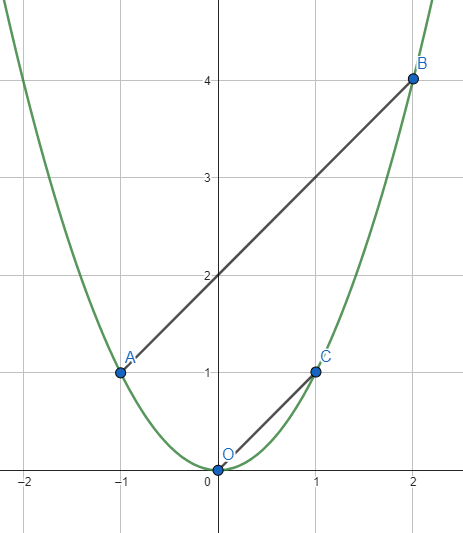
\includegraphics[width=0.3\linewidth]{img/parabella.png}
    \caption{}
\end{figure}

\begin{parts}
    \part Räkna ut lutningen på linjen $AB$.
    \part Räkna ut lutningen på linjen $OC$
    \part Visa att $a+b=c$
    \part[\medel] Vi ritar en till linje, $DE$, parallel med de första, där $D$ och $E$ är två punkter på parabeln.
    Visa att mittpunkterna på dessa tre parallella linjer ligger på en rät linje. 
\end{parts}